\documentclass[a4paper]{article}
\usepackage[utf8x]{inputenc}
\usepackage[portuguese]{babel}
\usepackage{graphicx}
\usepackage{a4wide}
\usepackage[pdftex,hidelinks]{hyperref}
\usepackage{float}
\usepackage{indentfirst}
\usepackage{subcaption}
\usepackage[cache=false]{minted}
\usepackage{amsmath}
\usepackage{listings}
\usepackage{color}

\definecolor{dkgreen}{rgb}{0,0.6,0}
\definecolor{gray}{rgb}{0.5,0.5,0.5}
\definecolor{mauve}{rgb}{0.58,0,0.82}

\lstset{frame=tb,
language=C++,
aboveskip=3mm,
belowskip=3mm,
showstringspaces=false,
columns=flexible,
basicstyle={\small\ttfamily},
numbers=none,
numberstyle=\tiny\color{gray},
keywordstyle=\color{blue},
commentstyle=\color{dkgreen},
stringstyle=\color{mauve},
breaklines=true,
breakatwhitespace=true,
tabsize=4
}

\newcommand{\x}{\times}

\begin{document}

\title{Computação Gráfica\\ Primitivas gráficas}
\author{Bárbara Cardoso (a80453) \and Marcio Sousa (a82400) \and Pedro Mendes (a79003)}
\date{\today}

\begin{titlepage}

    %título
    \thispagestyle{empty}
    \begin{center}
        \begin{minipage}{0.75\linewidth}
            \centering
            %engenharia logo
            
\includegraphics[width=0.4\textwidth]{eng.jpeg}\par\vspace{1cm}
            \vspace{1.5cm}
            %títulos
            \href{https://www.uminho.pt/PT}{\scshape\LARGE Universidade do Minho} \par
            \vspace{1cm}
            \href{https://www.di.uminho.pt/}{\scshape\Large Departamento de Informática} \par
            \vspace{1.5cm}

            \maketitle
        \end{minipage}
    \end{center}

\end{titlepage}

\tableofcontents

\pagebreak

\section{Introdução}
Este trabalho foi proposto no âmbito da unidade curricular de Computação Gráfica, e tem como objetivo desenvolver um motor gráfico genérico para representar objetos a 3 dimensões.

O projeto está dividido em várias fases, sendo que nesta primeira, serão implementadas algumas primitivas gráficas, como o plano, o paralelepípedo, a esfera e o cone e também uma primeira implementação de dois modos de Câmera.

\section{Arquitetura do Projecto}
Após analisar o problema, foi decidido que o projeto está dividido em dois executáveis, o \texttt{generator} e o \texttt{engine}. Para além destes, temos também na nossa arquitetura uma biblioteca comum aos dois.

\subsection{Common}

Aqui está apenas definido um \texttt{Point.cpp/hpp} que representa um ponto no espaço 3D.

\begin{minted}{C++}
    class Point {
        private:
        float _x, _y, _z;
        // -- snip -- /
    }
\end{minted}

\subsection{Engine}

Este modulo é composto pelo \texttt{model.cpp/hpp} que representa cada modelo, ou seja, o conjunto de pontos que define cada um dos modelos, e disponibilizando também um método para os desenhar. E a \texttt{main.cpp} que carrega todos os ficheiros especificados no ficheiro \texttt{config.xml} e desenha-os no ecrã. Esta define também a lógica que controla a câmera.

O algoritmo de desenho é simples. Primeiro todos os modelos do ficheiro de configuração são carregados para memoria sobre a forma de \texttt{Model}s. De seguida cada um destes modelos é renderizado no ecrã, chamando \texttt{glVertex3f} para cada um dos seus pontos, pela ordem em que foram lidos, e, por fim, inicia-se o \textit{loop} do \textit{glut}. Desta forma os modelos são carregados apenas uma vez para memória.

\subsection{Generator}

Este modulo é composto pelo \texttt{generator.cpp/hpp} que disponibiliza métodos para gerar os pontos necessários para desenhar as 4 primitivas geométricas e a \texttt{main.cpp} que interpreta os argumentos da linha de comandos para chamar estes métodos e produzir um ficheiro com estes.

O trabalho feito por este modulo é explicado em mais detalhe na secção~\ref{sec:primitivas}.

\section{Primitivas}\label{sec:primitivas}

Para esta fase do projeto foram desenhadas quatro figuras, contando com um plano, um cubo, uma esfera e um cone. Serão, em seguida, apresentados os algoritmos para o cálculo dos pontos necessários para desenhar cada uma destas primitivas, bem como uma contextualização com as premissas utilizadas durante o raciocínio, quando necessário.

\subsection{Plano}
\begin{figure}[H]
    \centering
    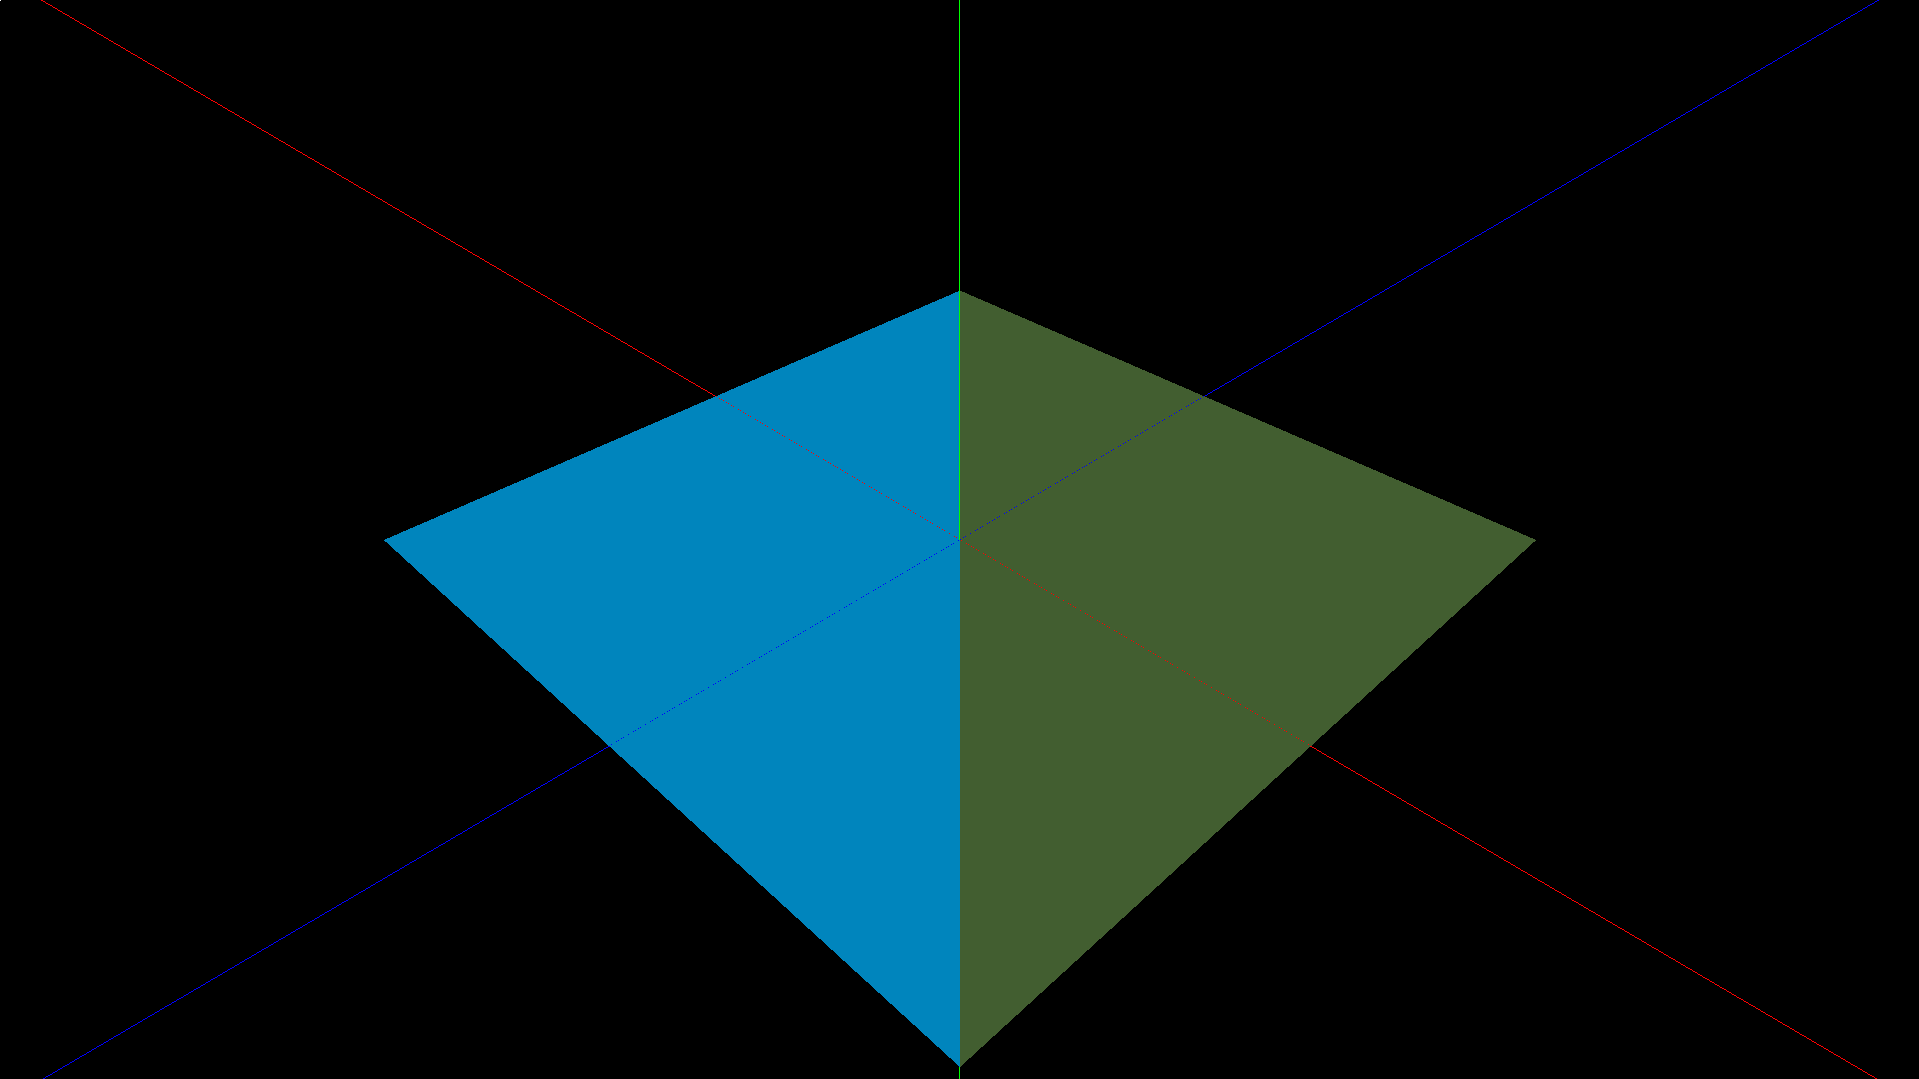
\includegraphics[width=\textwidth]{plane.png}
    \caption{Plano: Comprimento de Lado: 10}
\end{figure}

O plano é uma figura de extrema simplicidade, composto apenas por 6 pontos que formam 2 triângulos, que por sua vez darão origem ao plano em XoZ.


É recebido como parâmetro o comprimento do lado do quadrado em questão, que será usado para calcular os pontos. Sendo que este plano está centrado na origem, cada um dos pontos é calculado da seguinte forma:

\begin{figure}[H]
    \centering
    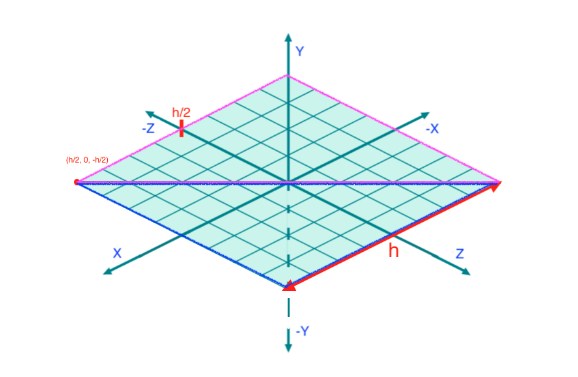
\includegraphics[width=0.6\textwidth]{esquemaPlano.PNG}
    \caption{Esquema do Plano.}
\end{figure}

Para definir o triângulo superior:

\[(h/2,\quad 0, \quad h/2)\]
\[(-h/2,\quad  0, \quad -h/2)\]
\[(-h/2,\quad  0, \quad h/2)\]

Para definir o triângulo inferior:

\[(-h/2, \quad 0, \quad -h/2)\]
\[(h/2, \quad  0, \quad  h/2)\]
\[(h/2, \quad  0, \quad -h/2)\]

Com base em tudo referido até agora, temos então o algoritmo usado para o cálculo dos pontos.


\subsection{Paralelepípedo}
\begin{figure}[H]
    \centering
    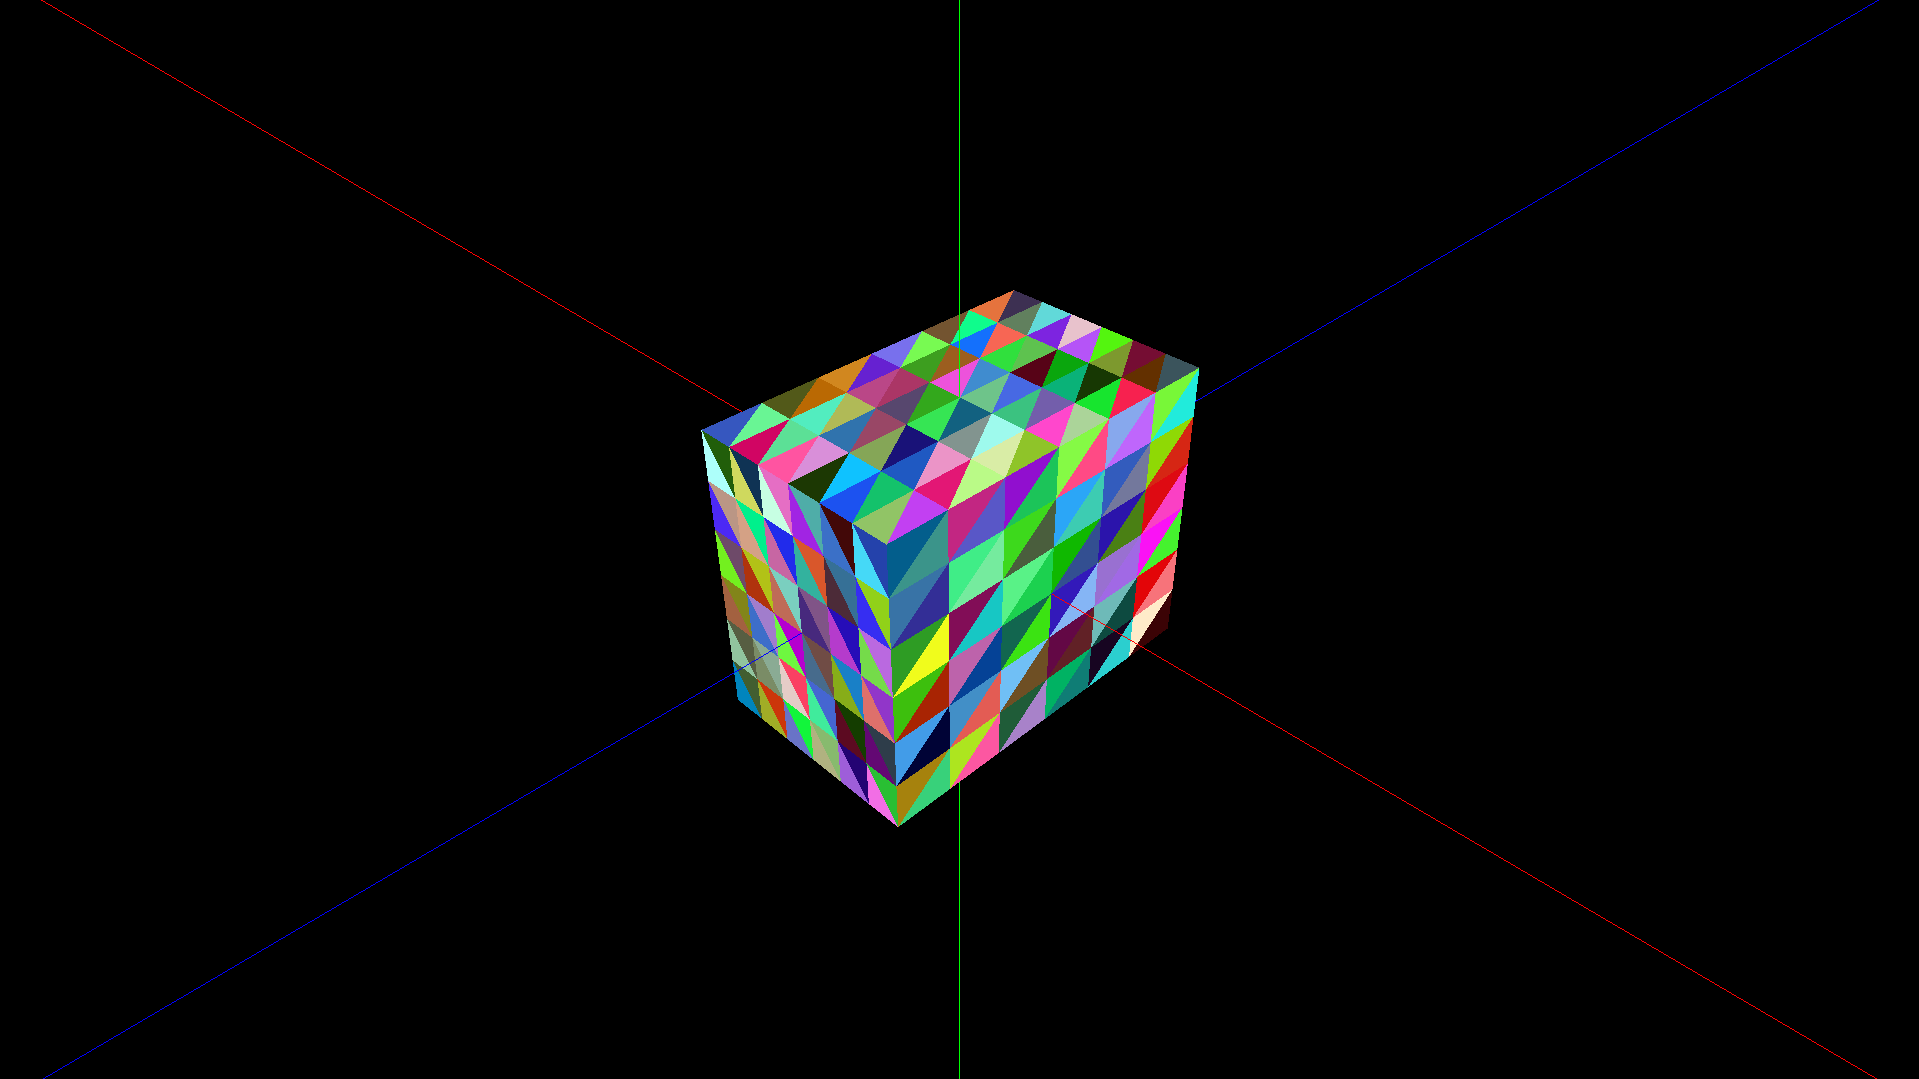
\includegraphics[width=\textwidth]{box.png}
    \caption{Paralelepípedo: x: 3, y: 4, z: 5, Divisões: 6}
\end{figure}

Um paralelepípedo é formado por 6 faces, sendo cada face formada por $divisions^2$ quadrados, sendo cada um desses quadrados formado por dois triângulos. Estas divisões são utilizadas para iterar sobre todas as superfícies do paralelepípedo, sendo esta distância entre divisões usada para calcular o próximo ponto baseado no ponto `atual'.

Tendo o paralelepípedo centrado na origem por motivos de facilidade de cálculos, calculamos:

\[X_{axis} = x / 2\]
\[Y_{axis} = y / 2\]
\[Z_{axis} = z / 2\]

como `valores máximos' que podem ser tomados por cada uma das coordenadas dos pontos que constituem o paralelepípedo, e

\[X_{spacing} = x / divisions\]
\[Y_{spacing} = y / divisions\]
\[Z_{spacing} = z / divisions\]

como sendo os valores que, tal como o nome indica, correspondem ao espaçamento entre divisões para cada eixo.

Para calcular todos os pontos foi feito uso do seguinte algoritmo:


\subsection{Esfera}

\begin{figure}[H]
    \centering
    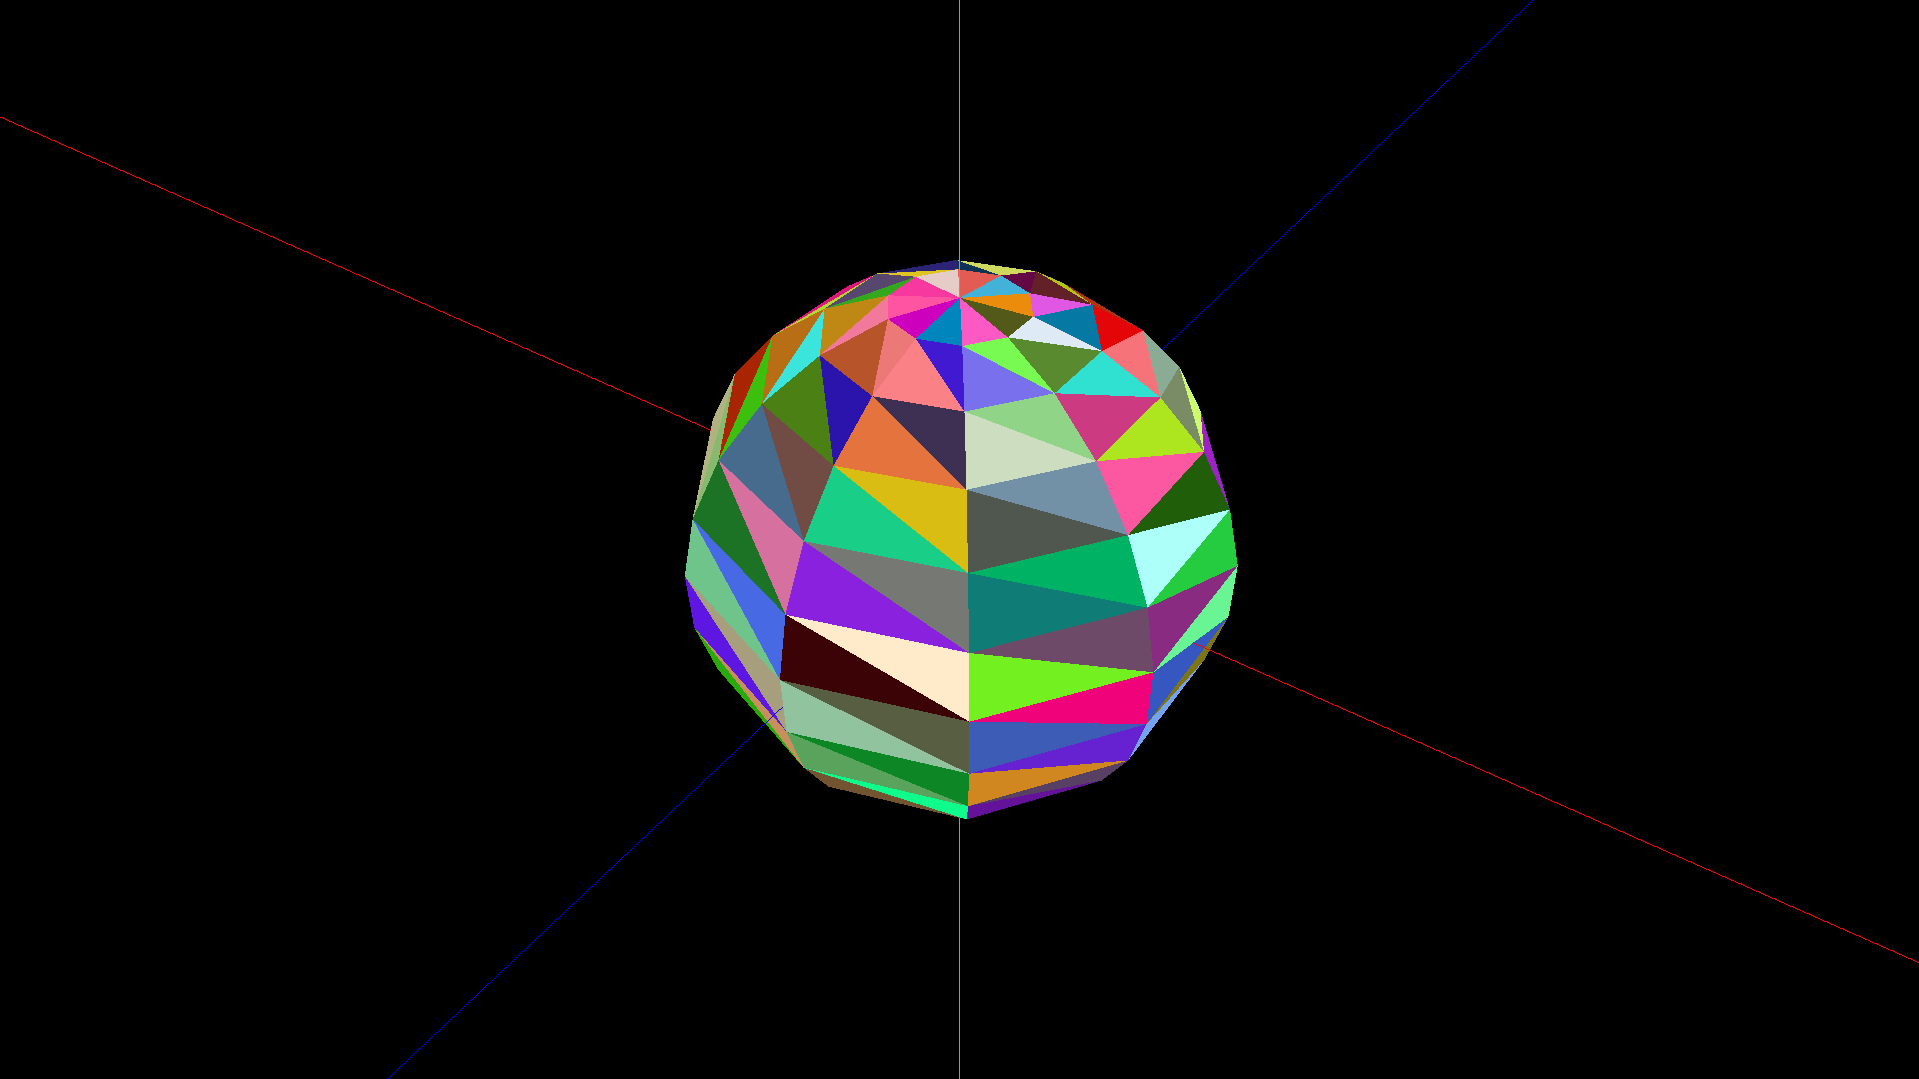
\includegraphics[width=\textwidth]{sphere.png}
    \caption{Esfera: Raio: 3, \textit{Slices}: 10, \textit{Stacks}: 7}
\end{figure}

Uma esfera é dividida em stacks e slices, que serão usadas para iterar a toda a volta da mesma. A interseção entre as slices e as stacks forma retângulos, e cada um desses retângulos será formado por dois triângulos.


Para a criação da esfera serão usadas coordenadas esféricas devido à facilidade que proporcionam no caso em questão. Assim sendo, são necessárias duas variáveis para representar os dois ângulos que constituem este tipo de coordenadas, \texttt{Phi} e \texttt{Theta}, utilizadas na iteração.

\begin{figure}[H]
    \centering
    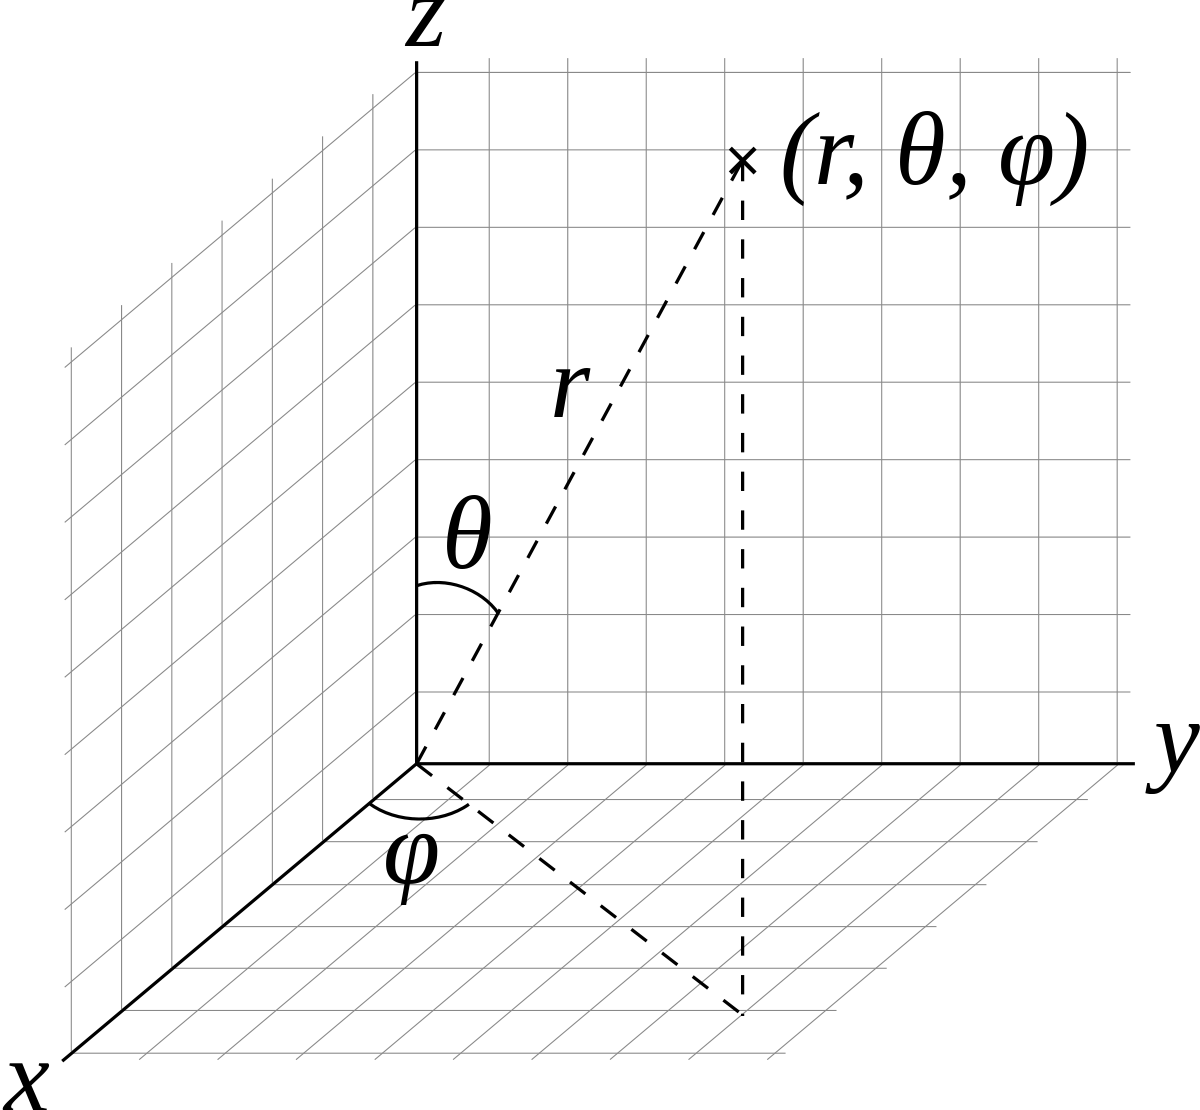
\includegraphics[width=0.5\textwidth]{coords.png}
    \caption{Coordenadas esféricas.}
\end{figure}

Para o cálculo das coordenadas de cada ponto será também necessário calcular a stack e slice em que se encontram atualmente as iterações, \texttt{currentStack} e \texttt{currentSlice} que serão calculadas da seguinte forma:

\[currentStack = \theta \x \theta_{Movement}\]
\[currentSlice = \phi \x \phi_{Movement}\]


As variáveis $\theta_{Movement}$ e $\phi_{Movement}$ correspondem, respetivamente, à distância entre Stacks e à distância entre Slices.

\[\phi_{Movement} = 2\pi / slices\]
\[\theta_{Movement} = \pi / stacks\]


Para utilizar coordenadas esféricas, o X, Y e Z devem ser alterados, passando a ser:

\[x = radius \x \sin(theta) \x \sin(\phi)\]
\[y = radius \x \cos(theta)\]
\[z = radius \x \sin(theta) \x \cos(\phi)\]

O algoritmo de cálculo dos pontos para desenhar uma esfera é a seguir apresentado.


\subsection{Cone}

\begin{figure}[H]
    \centering
    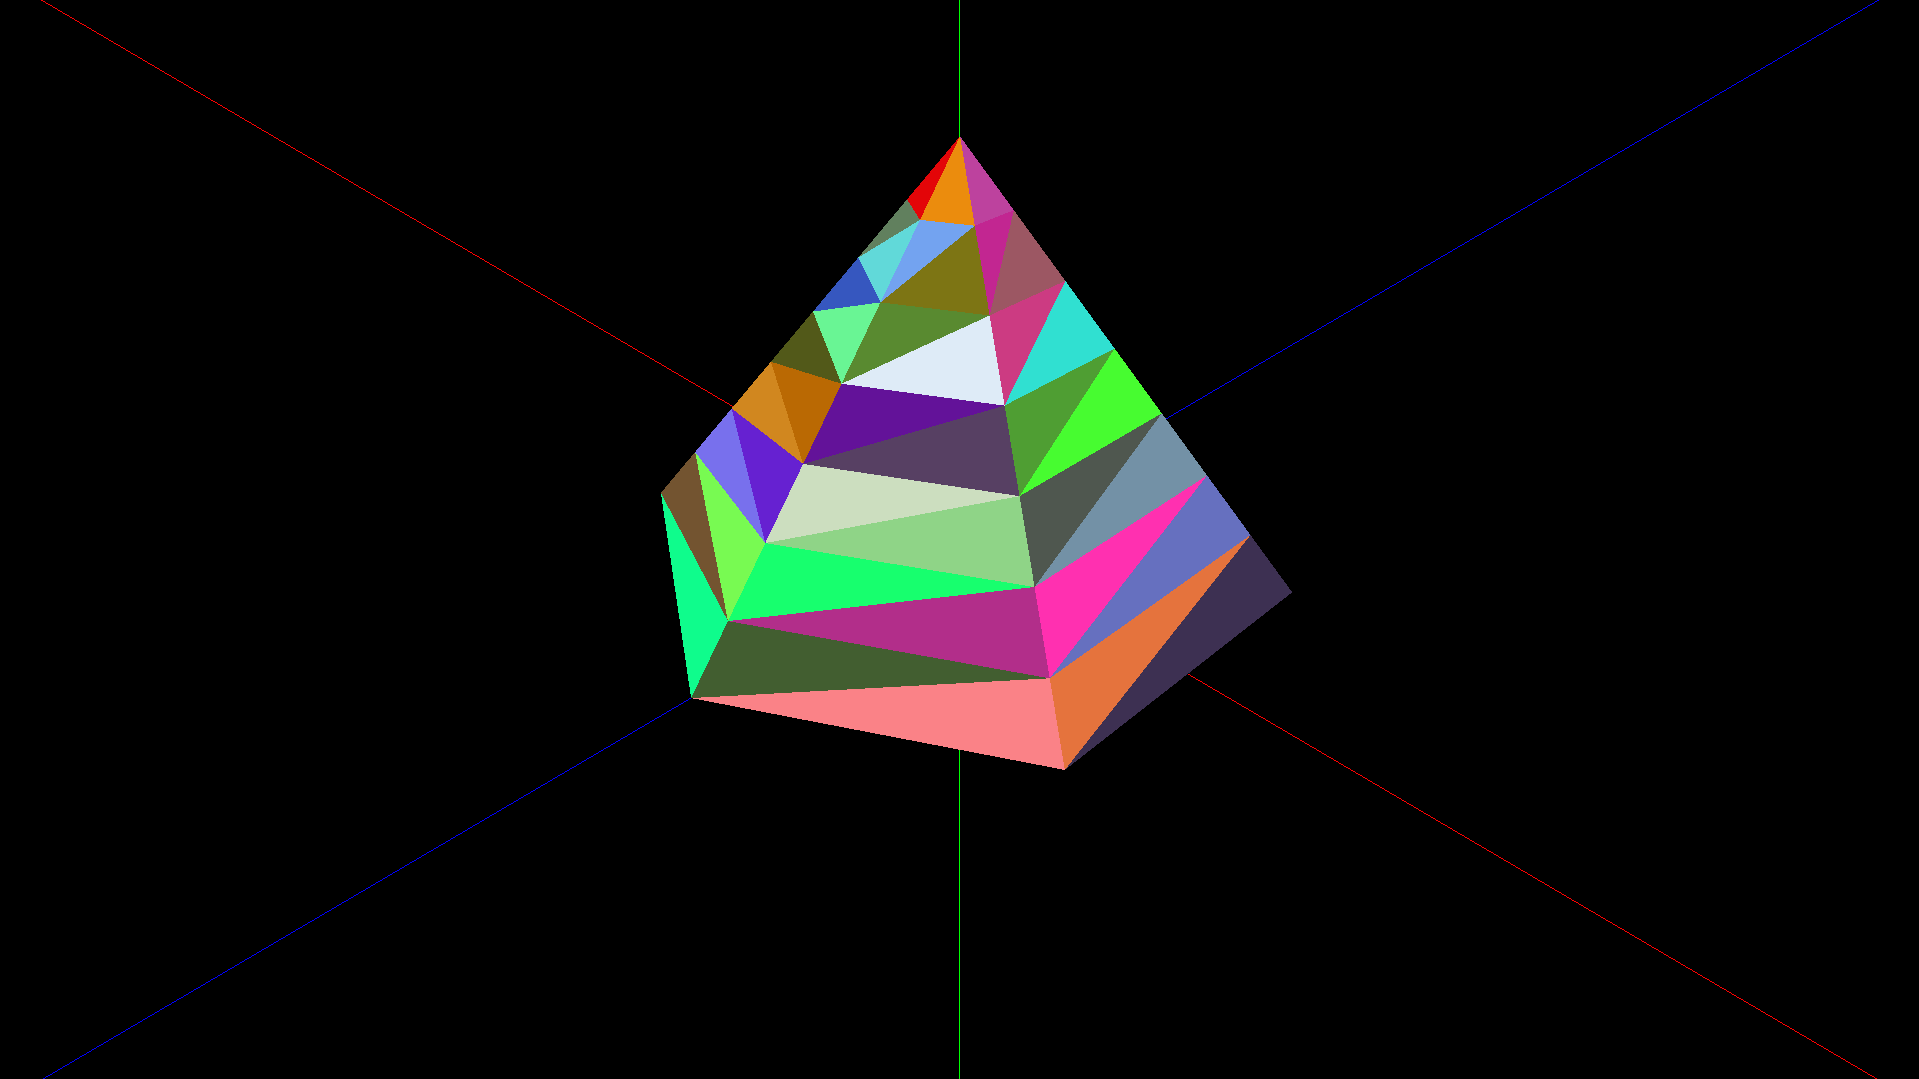
\includegraphics[width=\textwidth]{cone.png}
    \caption{Cone: Raio: 4, Altura: 5, \textit{Slices}: 6, \textit{Stacks}: 7}
\end{figure}

O cone tem a base sobre o eixo XoZ, centrada na origem, e é dividido em stacks e slices. A função geradora dos pontos do cone recebe como parâmetros o raio, a altura, o número de slices e o número de stacks.

São declaradas três variáveis, $\phi$, $\theta$ e $stackSpacing$.

A primeira corresponde à divisão equivalente da base por cada slice.

\[\phi = (2 \pi) / slices\]

A segunda, $\theta$, é calculada dividindo o raio da base pelo numero de stacks, o que se traduz na prática a calcular o recuo do raio à medida que se sobe nas stacks.

\[\theta = radius / stacks\]

Por fim, $stackSpacing$, tal como o nome indica, corresponde à distância entre cada stack, o *  `stack shift', e é calculado dividindo a altura pelo número de stacks.


\[stackSpacing = height / stacks\]


O desenho do cone em si foi dividido em 3 fases: Base, Topo e a zona em volta, e tal como na esfera, são utilizadas coordenadas esféricas.

\begin{figure}[H]
    \centering
    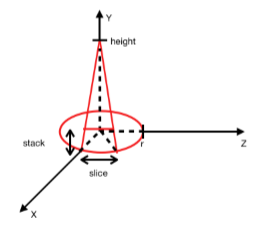
\includegraphics[width=0.5\textwidth]{coneEsquema.PNG}
    \caption{Esquema do cone.}
\end{figure}

Para a base, quando estamos na primeira stack, em cada iteração é desenhado um triângulo, e conjunto destes triângulos desenhados formarão a base concêntrica na origem quando tiverem sido executadas todas as iterações. Utilizando coordenadas esféricas chegamos às seguintes coordenadas:

 \[\Big(0, 0, 0\Big)\]
 \[\Big(radius \x \sin(\phi (k+1)), 0, radius \x \cos(\phi (k+1))\Big)\]
 \[\Big(radius \x \sin(\phi k), 0, radius \x \cos(\phi k)\Big)\]

sendo que $k$ toma valores entre $0$ e $slices-1$. Quando temos $\phi (k+1)$ representa o próximo valor de $\phi$.

O topo é desenhado no fim, para completar a "ponta" do cone, então, quando estamos na penúltima stack (a última é o vértice do cone), são desenhados triângulos a toda a volta que partilham um ponto em comum (o vértice), um por cada slice. Utilizando coordenadas esféricas chegamos às seguintes coordenadas:

\[\Big((radius - \theta i) \x \sin(\phi k), i \x stackSpacing, (radius - \theta i) \x \cos(\phi k)\Big)\]
\[\Big((radius - \theta i) \x \sin(\phi (k + 1)), i \x stackSpacing, (radius - \theta i) \x \cos(\phi (k + 1))\Big)\]
\[\Big(0, stacks \x stackSpacing, 0\Big)\]

Para os lados, com exceção do topo, serão desenhados retângulos formados por dois triângulos cada um, e serão esses retângulos que constituem o cone até chegar ao topo. Chegamos às seguintes coordenadas:

\[\Big(i(radius - \theta) \x \sin(\phi k), i \x stackSpacing, i(radius - \theta) \x \cos(\phi k)\Big)\]
\[\Big(i(radius - \theta) \x \sin(\phi (k + 1)), i \x stackSpacing, (radius - \theta i) \x \cos(\phi (k + 1))\Big)\]
\[\Big((radius - \theta (i + 1)) \x \sin(\phi k), (i + 1) \x stackSpacing, (radius - \theta (i + 1)) \x \cos(\phi k)\Big)\]

\section{Camera}
A Camera pode ser utilizada em dois modos diferentes, o modo \textit{Explorer mode} e o modo \textit{FPS mode}, que podem ser alternados durante a execução do engine.

\subsection{Explorer Mode}

Neste modo o movimento da camera é descrito por uma superfície esférica, na qual o utilizador se movimenta enquanto mantém, sempre, o seu olhar fixo na origem do referencial. O raio desta superfície esférica é que define a distância até ao centro, podendo ser aumentado para afastar o utilizador do centro do espaço 3d, ou diminuído para o aproximar.

\subsubsection{Controlos \textit{(key bindings)}}

\begin{itemize}
    \item \texttt{H}: Move no plano xz no sentido ao dos ponteiros do relógio.
    \item \texttt{J}: Desce.
    \item \texttt{K}: Sobe.
    \item \texttt{L}: Move no plano xz no sentido contrário ao dos ponteiros do relógio.
    \item \texttt{I}: Reduz o raio da esfera.
    \item \texttt{O}: Aumenta o raio da esfera.
\end{itemize}

\subsection{FPS Mode}

Neste modo a posição da câmera no espaço 3d é completamente livre, assim o utilizador pode mover-se em linha reta em qualquer direção. Pode também alterar o ponto para o qual está a olhar na horizontal e na vertical.

\subsubsection{Controlos \textit{(key bindings)}}

\begin{itemize}
    \item \texttt{W}: Move para a frente.
    \item \texttt{A}: Move para a esquerda.
    \item \texttt{S}: Move para trás.
    \item \texttt{D}: Move para a direita.
    \item \texttt{H}: Olha para a esquerda.
    \item \texttt{J}: Olha para baixo.
    \item \texttt{K}: Olha para cima.
    \item \texttt{L}: Olha para a direita.
    \item \texttt{G}: Desce.
    \item \texttt{Shift+G}: Sobe.
\end{itemize}

\subsection{Transição de modos da câmera}

Para que a transição seja o mais suave possível foi necessário recorrer à conversão de um sistema de coordenadas para o outro.

Quando a câmera se encontra no modo \textit{Explorer}, a sua posição é determinada através do vetor definido pelos ângulos $\alpha$ e $\beta$ e através da sua distância à origem. O ponto para onde a câmera olha é a origem. Ou seja, para efetuar a transição para o modo \textit{FPS} foi necessário encontrar um vetor que quando aplicado na posição da câmera, esta fique a olhar para a origem.

\begin{figure}[H]
    \[
        \alpha_f =
        \begin{cases}
            \alpha_e + \pi & \quad \text{se } \alpha_e < 0\\
            \alpha_e - \pi & \quad \text{caso contrário}
        \end{cases}
    \]
    \[
        \beta_f = -\beta_e
    \]
    \caption{Transição de \textit{Explorer} para \textit{FPS}.}
\end{figure}

Quando a câmera se encontra no modo \textit{FPS} é necessário encontrar os ângulos $\alpha$ e $\beta$ e também o raio. Estes valores definem o vetor correspondente às coordenadas (\texttt{(x,y,z)}) da câmera no momento da transição.

\begin{figure}[H]
    \[
        \alpha_e =
        \begin{cases}
            \arctan(x / z)       & \quad \text{se } z < 0\\
            \arctan(x / z) + \pi & \quad \text{caso contrario}
        \end{cases}
    \]
    \[
        \beta_e = \arcsin\bigg(\frac{y}{\sqrt{x^2 + y^2 + z^2}}\bigg)\\
    \]
    \[
        radius = \sqrt{x^2 + y^2 + z^2}
    \]
    \caption{Transição de \textit{FPS} para \textit{Explorer}.}
\end{figure}

\subsection{Outros controlos \textit{(key bindings)}}

\begin{itemize}
    \item \texttt{+}: Aumenta a escala de todos os modelos.
    \item \texttt{-}: Diminui a escala de todos os modelos.
    \item \texttt{V}: Muda o modo da câmera.
    \item \texttt{Q}: Termina o programa.
\end{itemize}

\section{Gestão de memória}

Foi utilizada a ferramenta \texttt{Valgrind} para garantir que não havia \textit{leak}s de memória.

Para o gerador foram testadas todas as primitivas:


\begin{verbatim}
==14866== Command: target/generator/generator plane.3d plane 10
==14866==
==14866==
==14866== HEAP SUMMARY:
==14866==     in use at exit: 0 bytes in 0 blocks
==14866==   total heap usage: 54 allocs, 54 frees, 83,619 bytes allocated
==14866==
==14866== All heap blocks were freed -- no leaks are possible
==14866==
==14866== For counts of detected and suppressed errors, rerun with: -v
==14866== ERROR SUMMARY: 0 errors from 0 contexts (suppressed: 0 from 0)
\end{verbatim}

\begin{verbatim}
==14867== Command: target/generator/generator box.3d box 20 30 40 6
==14867==
==14867==
==14867== HEAP SUMMARY:
==14867==     in use at exit: 0 bytes in 0 blocks
==14867==   total heap usage: 542 allocs, 542 frees, 263,139 bytes allocated
==14867==
==14867== All heap blocks were freed -- no leaks are possible
==14867==
==14867== For counts of detected and suppressed errors, rerun with: -v
==14867== ERROR SUMMARY: 0 errors from 0 contexts (suppressed: 0 from 0)
\end{verbatim}

\begin{verbatim}
==14868== Command: target/generator/generator sphere.3d sphere 10 100 200
==14868==
==14868==
==14868== HEAP SUMMARY:
==14868==     in use at exit: 0 bytes in 0 blocks
==14868==   total heap usage: 239,468 allocs, 239,468 frees, 68,346,015 bytes allocated
==14868==
==14868== All heap blocks were freed -- no leaks are possible
==14868==
==14868== For counts of detected and suppressed errors, rerun with: -v
==14868== ERROR SUMMARY: 0 errors from 0 contexts (suppressed: 0 from 0)
\end{verbatim}

\begin{verbatim}
==14871== Command: target/generator/generator cone.3d cone 10 6 100 200
==14871==
==14871==
==14871== HEAP SUMMARY:
==14871==     in use at exit: 0 bytes in 0 blocks
==14871==   total heap usage: 238,474 allocs, 238,474 frees, 68,075,587 bytes allocated
==14871==
==14871== All heap blocks were freed -- no leaks are possible
==14871==
==14871== For counts of detected and suppressed errors, rerun with: -v
==14871== ERROR SUMMARY: 0 errors from 0 contexts (suppressed: 0 from 0)
\end{verbatim}


E para o motor foi testado todo o código à exceção das rotinas do OpenGl:

\begin{verbatim}
==18205== Command: target/engine/engine
==18205==
==18205==
==18205== HEAP SUMMARY:
==18205==     in use at exit: 0 bytes in 0 blocks
==18205==   total heap usage: 18,726,897 allocs, 18,726,897 frees,
                                1,353,099,887 bytes allocated
==18205==
==18205== All heap blocks were freed -- no leaks are possible
==18205==
==18205== For counts of detected and suppressed errors, rerun with: -v
==18205== ERROR SUMMARY: 0 errors from 0 contexts (suppressed: 0 from 0)
\end{verbatim}


\section{Conclusões e Trabalho Futuro}
Em suma, todas as primitivas são geradas corretamente e o motor gráfico é capaz de as representar genericamente.

Futuramente, a câmera será melhorada para que se possa utilizar o rato no modo \textit{FPS}.

\end{document}

